\documentclass{standalone}
\usepackage{xcolor}
\usepackage{verbatim}
\usepackage[T1]{fontenc}
\usepackage{graphics}
\usepackage{hyperref}
\newcommand{\code}[1]{\texttt{#1}}
\newcommand{\R}{R}
\newcommand{\pkg}[1]{#1}
\newcommand{\CRANpkg}[1]{\pkg{#1}}%
\newcommand{\BIOpkg}[1]{\pkg{#1}}
\usepackage{amsmath,amssymb,array}
\usepackage{booktabs}
\usepackage{tikz}
\usetikzlibrary{positioning}
\usepackage{bm}

\begin{document}
\nopagecolor
	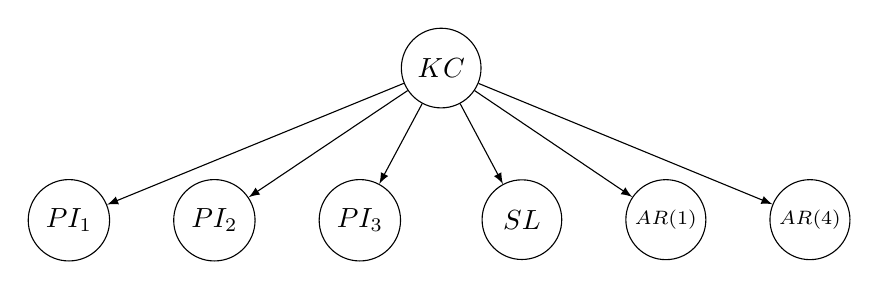
\begin{tikzpicture}
	\tikzstyle{main}=[circle, minimum size = 4mm, inner sep=2pt, text width=8mm,  draw =black, align=center, node distance = 8mm]
	\tikzstyle{connect}=[-latex]
	\tikzstyle{box}=[rectangle, draw=black!100]
	
	\node[main] (Y){$KC$};
	\node[main] (X3)[below left=12 mm and 3mm of Y] {$PI_3$};
	\node[main] (X2)[left=of X3] {$PI_2$};
	\node[main] (X1)[left=of X2] {$PI_1$};
	\node[main] (X4)[below right= 12 mm and 3mm of Y] {$SL$};
	\node[main] (X5)[right=of X4] {$\scriptstyle  AR(1)$};
	\node[main] (X6)[right=of X5] {$\scriptstyle  AR(4)$};
	\path (Y) edge [connect] (X1)
	(Y) edge [connect] (X2)
	(Y) edge [connect] (X3)
	(Y) edge [connect] (X4)
	(Y) edge [connect] (X5)
	(Y) edge [connect] (X6);
	
	\end{tikzpicture}
\end{document}
